% Literature review for the first meeting

\documentclass[a4paper,11pt,twoside]{article}
\usepackage[T1]{fontenc}
\usepackage[utf8]{inputenc}
\usepackage{color,dcolumn,graphicx,hyperref}
\usepackage{wrapfig}
\usepackage[top=2.5cm, bottom=2.5cm, left=2.5cm, right=2.5cm]{geometry}
\usepackage{setspace}
\onehalfspacing
\usepackage{scrextend}
\addtokomafont{labelinglabel}{\sffamily}
\usepackage[round]{natbib}
\bibliographystyle{abbrvnat}
\usepackage{tcolorbox}
\usepackage{filecontents}
\usepackage{csquotes}
\usepackage{epigraph}
\usepackage{ragged2e}
\usepackage{wrapfig}
\usepackage[font=small]{caption}
\hypersetup{
  colorlinks = true,
  allcolors=[rgb]{0,0.4,0.5},
}

%% Packages for Graphics & Figures
\usepackage{graphicx} %%For loading graphic files
\usepackage{float}

%% Math Packages
\usepackage{amsmath}
\usepackage{amsthm}
\usepackage{amsfonts}


\title{
  PhD project \\
  \bigskip
  Linking forest management and species distribution models: \\
  a theoretical approach under climate change
}

\author[1,*]{Willian Vieira}
\affil[1]{Département de Biologie, Université de Sherbrooke, Sherbrooke, Québec, Canada}
\affil[*]{w.vieiraw@gmail.com}
\date{}

\begin{document}

\maketitle

\begin{abstract}

\textbf{TODO}: \\
- Abiotic and biotic constraints \\
- Forest management and productivity \\
- Theoretical approach (SDM, Disturbance, resilience calculus, alternative stable state and early warning signals) \\
- All study case: Québec Forest ressource \\
- All methods \\
- Better description of thesis structure \\
- Abstract \\
- Short reference style \\
- Change \LaTeX color syntax in Atom

\end{abstract}

%logo
\vfill
\begin{figure}
\centering
\includegraphics[width=16cm]{img/logo.pdf}
\end{figure}
\thispagestyle{empty} %no page number in the first page
\clearpage

\thispagestyle{empty}
\tableofcontents
\clearpage

% START DOCUMENT

\begin{displayquote}
\centering\textit{Ecology may provide many of the answers — but only if it is holistic enough to incorporate the human element as part and parcel of the ecosystem.} \\ \RaggedLeft{\citep[p. 231]{Pfister1993}}
\end{displayquote}

\section{What is going on?}

Climate change is an increasing trending topic both in non-scientific \citep{Capstick2015} and scientific environment (Figure \ref{fig:fig1}), transforming our world as a metamorphosis of practice and acting \citep{Beck2016}.
According to IPCC \citep{Cubasch2013}, humans activities are contributing to increase the concentration of greenhouse gases, which can lead to increase the mean temperature and the strength of extreme climate events.
This global change has an impact in different biological processes, from local species constraints \citep[e.g. low regeneration][]{Treyger2011}, shift in species' range \citep{Boisvert-Marsh2014,Monleon2015} and in community composition \citep{Dieleman2015} to range retractions and extinction \citep{Thomas2006}, impacting biodiversity at different scales \citep{Penuelas2013}.

\begin{wrapfigure}{r}{0.38\textwidth}
    \centering
    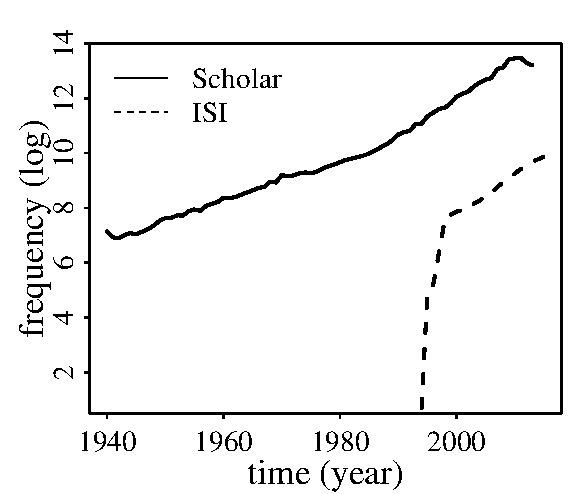
\includegraphics[width=0.38\textwidth]{img/fig1_em.pdf}
    \caption{Frequency of the keyword ``Climate change'' used in publications indexed on Google Scholar (1940 - 2013) and Web of Science (1994 - 2015)}
    \label{fig:fig1}
\end{wrapfigure}

Species distribution models (SDM; defined in section \ref{sdm}) is one of the most popular method to predict species' range shift under climate change, providing a wide range of applications, as in biodiversity conservation and management \citep{Guisan2005,Guisan2013}.
However, these models are generally phenomenological and  distributed at equilibrium with climate \citep[e.g.][]{Pigot2013}, being an issue when species observation does not reflect its niche \citep{Schurr2012}.
Furthermore, they do not consider important determinants of range limits as demography \citep{Louthan2015}, ecological constraints \citep{Wisz2013,Pigot2013} and species absences data \citep{Koshkina2017}, inducing non-accurately projection of the future spatial distribution of a species \citep{Tavecchia2016}.
Considering this determinants, trees' migration rate following climate change will be slower than predicted \citep{Bertrand2011,Sittaro2017}, increasing the climatic debt \citep{Bertrand2016}.

%Extinction debt is following climate debt?
The climatic debt is a measure of the lag (or disequilibrium) of plant communities with climate change, integrated in an environmental context \citep{Bertrand2016}.
\citet{Essl2015} has listed twelve mechanisms that contribute to delayed biodiversity responses, among them, changes appears at ecosystem (loss and degradation), community (secessional, biotic interaction, species removal and invasion) and population (evolutionary and adaptive) levels.
Physical changes cause biotic changes that directly and indirectly promotes species' persistence and/or species' migration \citep{Bertrand2016}.
This mechanisms of persistence (measured by resistance) and migration (measured by recovery) leads to a climate debt and migration credit, respectively \citep{Bertrand2016} but also a concept of resilience\footnotemark{} \citep{Oliver2015}.
Therefore, this lag under climate change promotes extinction debt, being a challenging for biodiversity conservation \citep{Kuussaari2009} and productivity \citep{Lasch2002}.
Identify the mechanisms shaping delayed biotic response of systems to environment, its resilience as well as alternatives to mitigate ecological constraints, is crucial to access the vulnerability of biodiversity to climate change and improve forecasts and biodiversity management \citep{Essl2015,Oliver2015,Bertrand2016}.

\footnotetext{Here I use \textbf{recovery resilience} (recovery time to equilibrium) and \textbf{resistance} to describe the whole mechanisms of ecological resilience (see why in section \ref{res})}

\section{Preliminary objectives}
%I call this section as ``preliminary'' because I am still trying to figure out possible gaps I will be interested in working on.
%I also believe that classifying my plan as preliminary will help me identify throughout my thesis the ``best'' route to finish it in a pleasurable and creative way.

The primary objective of my thesis is to study if forest management can increase the speed of transition (i.e. recovery resilience) from temperate to boreal forests observed in the North Eastern America.
To achieve, I will use theoretical models parameterized from a forest inventory database, focusing on tracking uncertainty using Bayesian approach.
As an outcome, I will create a decision make tool to improve management strategies that take climate change into account.

My PhD is based in four questions so far: \\
(i) Which mechanisms are affecting the delayed biotic response to climate change? What is the origin, direction and intensity of these mechanisms? \\
(ii) How can forest management affect these mechanisms to increase resilience and therefore speed up the response? \\
(iii) How these mechanisms interact at local and global scale? \\
(iv) How can these mechanisms be used to inform applied management to enhance the resilience and productivity?

\section{Mechanisms of delayed biotic response}

Mechanisms shaping delayed biotic response and ecological resilience act at different scales and usually they interact with each other across scales, which makes the process sometime difficult to track and therefore to mitigate.
Furthermore, there is a focus attention in mechanisms at the metapopulation level where local mechanisms are often ignored \citep{Hylander2013}; it creates a knowledge gap in understanding all the possibles mechanisms as well as its interactions.
In this context, I will start my thesis trying to identify how we can increase forest resilience by managing these mechanisms, or more specific, how to decrease the recovery time of a system from a disturbance to a steady state (theories described in section \ref{ta}).
Here, I present some mechanisms that may be affecting the delayed response to climate change, as well as forest resilience, in which may become possible topics I will be testing during my thesis using SDM approach, working both at local and large scale.

\subsection{Biotic Mechanisms}

Biotic mechanisms affect the delayed response from individual and population species to community level.
At the individual scale, the lifecycle elements of a species \textit{j}, represented by demography patters, is a mechanism able to alter the time response from environmental perturbations \citep{Bertrand2016}.
For example, species with a high growth rate will recover faster \citep{Grman2010}, in which we can expect a high recovery resilience; the allee effect can, however, induce the opposite effect by reducing mean vital rates \citep{Dennis2002}.
In parallel, the sensitivity of a species also plays an important role in its response to perturbations \citep{Oliver2015,Bertrand2016}; sensitive species respond faster and also has a high recovery resilience.
In other hands, both species (with high growth and sensitivity) have a low resistance to environmental changes; it means that, if they have a low adaptive phenotypic plasticity, they will not be able to survive.
Phenotypic plasticity is the (behaviour, morphology or physiology) change of an individual in response to the environmental change \citep{Price2003}; this adaptive process, together with evolutionary adaptation \citep{Bertrand2016} is a mechanism that increase both species resistance and recovery resilience \citep{Essl2015,Oliver2015}.

In a metapopulation level, high genetic variability increase both resistance and recovery resilience of species \citep{Hylander2013,Oliver2015}.
Dispersal mechanisms can affect genetic variability (the low exchange between individuals, the low variability), in which together with the low dispersal ability of forest species, can lead to an increase in climate debt \citep{Hylander2013,Bertrand2016}.
Further than dispersion, the effective population size also affect genetic variability \citep{Oliver2015}, where small populations increase the likelihood for inbreeding and hence the extinction risk \citep{Nieminen2001}.
These individual and populational mechanisms are, however, rarely affecting species alone; instated there must be interactions between them \citep{Hylander2013}, as well as extra mechanisms acting from different scales and origins.

Because different species are normally distributed together limiting one another \citep{clark2014}, consider biotic interactions across trophic levels is essential to predict species distribution \citep{VanderPutten2010}, as well as understand its impact on delayed biodiversity response \citep{Essl2015}.
For example, trees competition for soil nitrogen has amplified climate debt, but it varies depending on the resource \citep{Bertrand2016}.
Species interaction itself is determined by multiple mechanisms \citep[for an overview]{Louthan2015} and a shift from single-species distribution to community distribution is suggested \citep{Cazelles2016}.
In a interaction network, the loss of one specie can lead to cascade extinction, reducing network stability \citep{Dunne2002} and, if the specie is sensitive, the functional resistance.
In addition, the recovery resilience and resistance of a system depend if different species perform complementary functions (i.e. functional redundancy) or respond in different ways to perturbation \citep{Winfree2009}; it means resistance increase when the network are dominated by non-specialized interactions \citep{Oliver2015}.

\subsection{Abiotic Mechanisms}

Abiotic or physical mechanisms can also shape delayed biotic response and ecological resilience, in which a better quality environment will support plant development and therefore its resistance to perturbation.
At the soil level, for example, nitrogen availability can limite the growth of trees \citep{Sullivan2013} and high nitrogen content and low acidity soils impact both species sensitivity and competition, amplifying the climate debt \citep{Bertrand2016}.
Likewise, less suitable climates constrained demographic strategies, increasing retrogression and vulberability of plant species \citep{Csergo2017}  and increase in the severity of climate events inflated climate debt \citep{Bertrand2016}.

Because environmental heterogeneity increases overall species richness \citep{Stein2014}, the resistance of a system is enhanced by functional redundancy \citep{Oliver2015}.
Environmental heterogeneity also provides a range of microclimatic refugia, which allow species to persist locally to climate changes \citep{Maclean2015}; however, \citet{Bertrand2016} found that microclimatic refugia plays a minor role comparing with other determinants of climatic debt.
Ecosystem loss and degradation are mechanisms that contribute to loss and decrease in species diversity \citep{Essl2015}, as well as decrease landscape connection.
Disconnected landscapes have then slow recovery resilience of a system after perturbation, i.e., low functional connectivity \citep{Oliver2015}.

- Disturbance
Is important according to Essl but was important according to Bertrand

\textit{Human-induced drivers} \\
- Land use by Goring and William 2017 \\
see Cabral 2017

\section{Forest management}

 L’article de Bottero et al. rapporte une augmentation de la résistance à la sécheresse lorsqu’on réduit la densité d’un peuplement forestier. Chase et al. précisent que ce gain en productivité serait attribuable à des conditions d’humidité du sol plus favorables aux printemps.  Sohn et al. rajoute que les ÉPC vont, en fait, augmenter la plasticité des réponses physiologiques de l’arbre aux changements environnementaux.  Par contre, D’Amato et al. préviennent que ce gain en résistance à la sécheresse disparait lorsque les peuplements prennent de l’âge.

Lessons from large-scale environmental management successes, for example measures to reduce the causes of ‘acid rain’ (Fowler et al. 1982), show that action at local and global scales must complement each other if wide-scale environmental management efforts are to be successful.
Present some motivations, advantages and disadvantages in considering forest management. (in Rhodes 2015)

It is clear that some factors will be more amenable to management (e.g., population-level genetic variability, landscape structure
[18,31]) than others (e.g., environmental sensitivity of individual species, presence of alternative stable states). In Olivier 2015

Four major strategies are available to mitigate carbon emissions through forestry activities: (i) to increase forested land area through reforestation (6), (ii) to increase the carbon density of existing forests at both stand and landscape scales, (iii) to expand the use of forest products that sustainably replace fossil-fuel CO2 emissions, and (iv) to reduce emissions from deforestation and degradation. in Managing forests for climate change mitigation (Science)

http://onlinelibrary.wiley.com/doi/10.1111/j.1752-4571.2010.00157.x/full \\
http://www.sciencedirect.com/science/article/pii/S0006320715301762

Interesting argument about who should peak do winners from \citet{Webster2017}. They say that \textit{Predict-and-prescribe management may erode diversity by focusing on ‘winners’}.

Forest management in a theoretical view was actually not very much explored and so I consider it a kind of gap we should better explore. Read \citet{Becknell2015} for an overview.

paper:Temporal stability in forest productivity increases with tree diversity due to asynchrony in species dynamics

However, this translation is limited by significant knowledge gaps including the following: (i) difficulties in detecting changes in resilience (Batt et al. 2013), (ii) a lack of evidence and agreement to support successful preventative management actions (Barrett et al. 2014) and (iii) the need to work across multiple geopolitical scales to achieve effective management (Servos et al. 2013). (In Rhodes 2015 at app eco)

\textbf{An operational model for resilience-based management}
Step 1: Detecting ecological sensitivity to pressures
Step 2: Developing more effective resilience-based management measures
Step 3: Achieving adaptive governance

\subsection{Forest productivity}
Robert m'a envoyé quelques articles qui discutent des facteurs qui contrôlent la dominance des arbustes éricacées en forêt boréale et de leur possible impacte sur la productivité forestière.

Lire toute le mail que je vais arriver avoir une bonne base pour discuter ici.

\section{Theoretical approach}\label{ta}

Read the section \textit{recent developments in predicting changes in species distribution} from \citet{Ehrlen2015}

\subsection{Range dynamics theory}

What theories can help us to describe species range under climate change?\\
How to integrate forest management in this theory?\\
-> Metapopulation dynamics theory <-

\subsection{Disturbance}
Pass through the main disturbance theories basing mainly in \citet{Pulsford2016}

\subsection{Resilience}\label{res}

A classical definition of resilience in ecology is the ability of ecosystems to absorb changes and still persist \citep{Holling1973}.
The concept was further developed in other context (e.g. social-ecological systems), and a more contemporary definition considers resilience as (i) the amount of disturbance the system can absorb, (ii) the degree the system is able to self-organize and (iii) the degree of learning capacity to adapt to disturbance \citep{Cumming2011}.
We have therefore two concepts, the time to \textbf{recovery} to stability and accommodated external changes \citep{pimm1984,Folke2002} and the \textbf{resistance} of a particular ecological state to change \citep{Peterson1998}.
Although \citet{Oliver2015} treat both resistance and recovery as related aspects of resilience, I prefer to keep these concepts separated in (i) recovery resilience (or engineering resilience) and (ii) resistance where both are englobed in ecological resilience \citep{Hodgson2015,Nimmo2015}.
Ecological resilience can be affected by different mechanisms from species to landscape levels, but biodiversity shows to be crucial to maintain long-term resilience of ecosystem services \citep{Oliver2015}.

It is also important to not confuse recovery resilience with stability of a system.
Recovery resilience is the rate and extent of ``restoration'' of a system while stability is when the system maintains stable following small perturbations over time.
Before introduce the method to calculate recovery resilience, we must know what is the equilibrium and stability (\hyperlink{box1}{Box 1}) of a system, as well as these measures are relative and careful must be taken when choosing \textit{resilience of what to what} \citep{Carpenter2001}.

\begin{tcolorbox}
\hypertarget{box1}{Box 1}. Equilibrium and Stability
\begin{align}
E &= mc^2 & \text{Formula of the universe}
\end{align}
\end{tcolorbox}

\begin{tcolorbox}
\hypertarget{box2}{Box 2}. Environmental transition (see Oliver2015)
\begin{align}
E &= mc^2 & \text{Formula of the universe}
\end{align}
\end{tcolorbox}

\textbf{(iii)} But how to calculate it in a analytical way?
To implement the results from these or other studies in management projects, it is necessary to disentangle the many meanings and measures of resilience and related stability concepts (In Mori at TREE).
Now introduce the calculus of $\lambda$ by Jacobian matrix (\hyperlink{box2}{Box 2}).
The Jacobian matrix has been used in different applications, from local models [...] to meta-ecosystems models \citep{Gravel2016}

\subsection{Transition period - Alternative Stable States?}
The existence of single equilibria is still often assumed in the literature, with critical implications for conservation and restoration. -- An important feature of this concept (resilience) is the emphasis on possible alternative system properties that are associated with renewal and reorganization after disturbance (In Mori 2016 at TREE)

Resilience-based management does not typically seek to increase the rate of return to an original state, which often implicitly assumes the existence of a single equilibrium, but instead recognizes that many natural systems could have multiple attractors [2, 3]. (In Mori 2016 at TREE)

\subsection{Early warnings?}

Resilience indicators: prospects and limitations for early warnings of regime shifts

For precautionary biodiversity management, the identification of robust early-warning signals (e.g., critical slowing down of recovery rates after perturbations) of approaching thresholds (tipping points) of losses of biodiversity or ecosystem services [9] is urgently needed (in Essl2015)

\section{Study case: the Quebec forest resource}

Explain here where I am going to work and also why I am choosing this area.

\section{Methods}

Here we see a briefly presentation of possible methods will be used in the thesis.

\subsection{Modeling}

Why and how modeling?\\
Morin et thuiller 2009:{What then are the best strategies for obtaining accurate predictions for changes in the distributions of deciduous temperate trees? At the scale of the geographic distribution of species, no experiments in situ can be reasonably carried out to predict possible range shifts (Woodward 1987). Modeling therefore appears the most feasible and efficient way to establish useful predictions (Lovejoy and Hannah 2005, Thuiller 2007), and several kinds of models have been developed during the previous decade for this purpose. As reviewed by Midgley et al. (2007), these models fall into two main classes: vegetation-type models (dynamic global vegetation models [DGVMs]) and species-specific models (niche-based and process-based).}

 L’article de Ashraf et Maclean porte sur un modèle de simulation de croissance d’arbres individuels en fonction des changements climatiques.  Leur modèle a été développé avec une technologie d’intelligence artificielle.

\subsubsection{Species Distribution Models}\label{sdm}

Nice resume about SDM in \citet{Moran-Ordonez2016}.

\subsubsection{Integral Projection Models}

the predictive powers of state and transition models are relatively low and their ability to deal with uncertainty is limited (Bashari, Smith and Bosch, 2008; Phillips, 2011).

\subsection{Bayesian approach}

\textit{I should be writing and not playing with \LaTeX}

\section{Thesis structure}

The first part of the thesis will be a general introduction where I will probably use a part of this document and present the big picture of my thesis.
I believe the introduction part of a thesis is an easy way to welcome the reader through my work, however in the actual context of digital era, no one really reads a whole PhD thesis and an efficient action to welcome and divulge my work is to publish it online.
An alternative approach to (sleepers) general introductions that, according to Stephen Heard\footnotemark{} no one reads but the author, is to publish it as a general papers in a scientific vulgarization journal.
In this way, my work will be easier to understand by both academics and general public, more accessible and the introduction part more useful.

The first chapter will try to answer the question \textit{How can forest management increase forest resilience to climate change?}.
The paper will first work with an analytical analysis in a SDM to understand the impact of forest management on increasing forest resilience.
Following, as an study case, we will test by sensitivity analysis the effect of forest management

In the second chapter I am going to build a landscape model that will consider both forest management and species interaction.

The third chapter I am going to build another model but in a local scale. \textit{I have to find a good biological reason for that}.

The fourth chapter will then integrate both landscape and local model into one. Here I will also track the uncertainty of the model by bayesian approach.

Finally, I will try to introduce my PhD reflexions into the big picture of ecology, management and ecosystem services. In an integrative and synthetic approach (more appropriate for a \textit{Forum} section), I will discuss my main results, its application and mainly the point of depart for future prosperous work.

\footnotetext{The three functions of a thesis, by Stephen Heard at the \href{https://scientistseessquirrel.wordpress.com}{Scientist Sees Squirrel}'s blog}

\clearpage
\bibliography{/users/wvieira/Documents/mendeley_bibtex/Thesis.bib}

\end{document}
